\section{问题四：变动电价下的滚动调度}

\subsection{未来价格的因果预测}

问题四的实际电价随日期和时槽变化。若在规划时直接读取当天未来真实价格，会产生明显的未来信息泄漏。本文对日期$d$、槽$t$的0时价格预测取过去30日同槽价格的中位数：
\begin{equation}
 \widehat c_{d,0,t}=\operatorname{median}\left\{c_{k,t}:\max(0,d-30)\le k<d\right\}.
 \label{eq:price-dayahead}
\end{equation}
首日没有历史时使用附件典型价格。日内时刻$h$重新规划时，计算当天已经实现的最近至多18槽价格偏差中位数 $b_{d,h}$，并按3小时尺度向未来衰减：
\begin{equation}
 \widehat c_{d,h,t}=\max\left\{10^{-4},\widehat c_{d,0,t}
 +b_{d,h}\exp\left[-\frac{t-t_h}{18}\right]\right\},\quad t\ge t_h .
 \label{eq:price-intraday}
\end{equation}
其中 $t_h=6h$。规划目标使用 $\widehat c$，真实 $c$ 仅用于合同和应急费用结算。图\ref{fig:q4-price}显示各月价格分布具有离散性和尾部，故单一月均价不足以描述调度机会；箱线图中的离群点均被保留。

中位数而非均值用于0时价格预测，是因为月内价格分布包含尾部，少数尖峰会明显拉动均值。该选择并不意味着忽略尖峰：安全供能仍由负荷和光伏分位轨迹控制，而价格中位数只决定有限电池能量在剩余时槽间的相对配置。当日偏差项使整体价格水平随已实现数据上移或下移，指数衰减则避免把刚刚发生的局部异常永久外推到全天。

在实际执行时，储能动作与真实价格的相关性只能作为事后描述，不能反向证明控制器预知价格。规划时可利用的是 $\widehat c_{d,h,t}$；真实 $c_{d,t}$ 在槽结束时进入结算。若实际高价尖峰未被历史中位数和已实现偏差预见，策略可能保留不足的SOC，这正是个别代表日有调账方案费用反而上升的可能机制之一。

\begin{figure}[H]
  \centering
  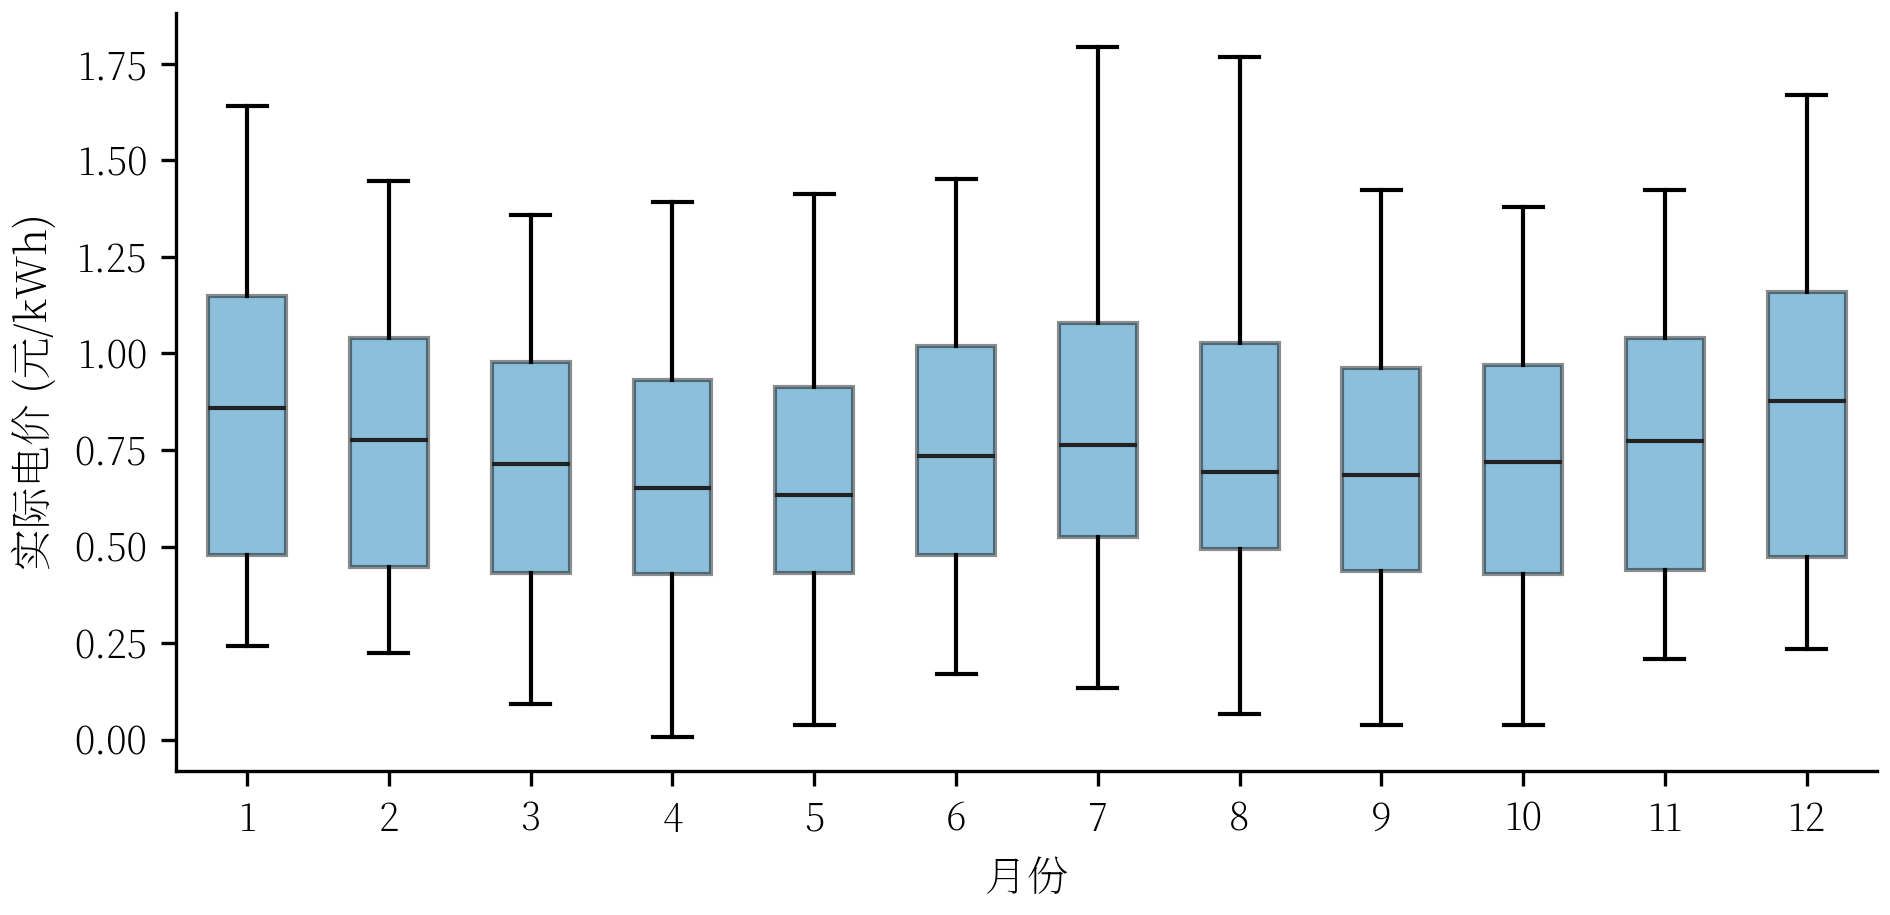
\includegraphics[width=0.98\textwidth]{figs/raw_q4_price_variability.png}
  \caption{2025年各月10分钟电价分布。箱体为四分位区间，须线为1.5倍四分位距，离群点未删除。}
  \label{fig:q4-price}
\end{figure}

\subsection{两种策略及结果}

问题四的无调账方案沿用问题二的相似日与分位轨迹，只把固定价目标替换为式\eqref{eq:price-dayahead}的预测价格；有调账方案沿用问题三的0、6、12、18时更新机制，并在每次滚动求解时使用式\eqref{eq:price-intraday}。两者执行层均只读取当前真实量，储能跨日连续。

表\ref{tab:q4main}给出正式统计结果。有调账方案比无调账方案节约 $2519380.1148$ 元，应急购电减少 $459960.1389\,\mathrm{kWh}$。若把问题二和问题三也纳入同一图，固定价与变价都呈现“有调账总体费用更低”的结果，见图\ref{fig:q4-result}。但是，固定价的$q2\to q3$和变价的$q4\_2\to q4\_3$都同时改变了信息与更新规则，不能当作单因素频率效应。

\begin{table}[H]
\centering
\caption{问题四两个方案的334日结果}
\label{tab:q4main}
\begin{tabular}{lrrrr}
\toprule
方案 & 现金费用/元 & 应急/kWh & 闲置合同/kWh & 弃光/kWh\\
\midrule
无调账 & 19,254,498.44 & 575,898.35 & 4,100,533.58 & 1,969,275.57\\
有调账 & 16,735,118.32 & 115,938.21 & 3,085,161.95 & 1,848,622.33\\
\bottomrule
\end{tabular}
\end{table}

\begin{figure}[H]
  \centering
  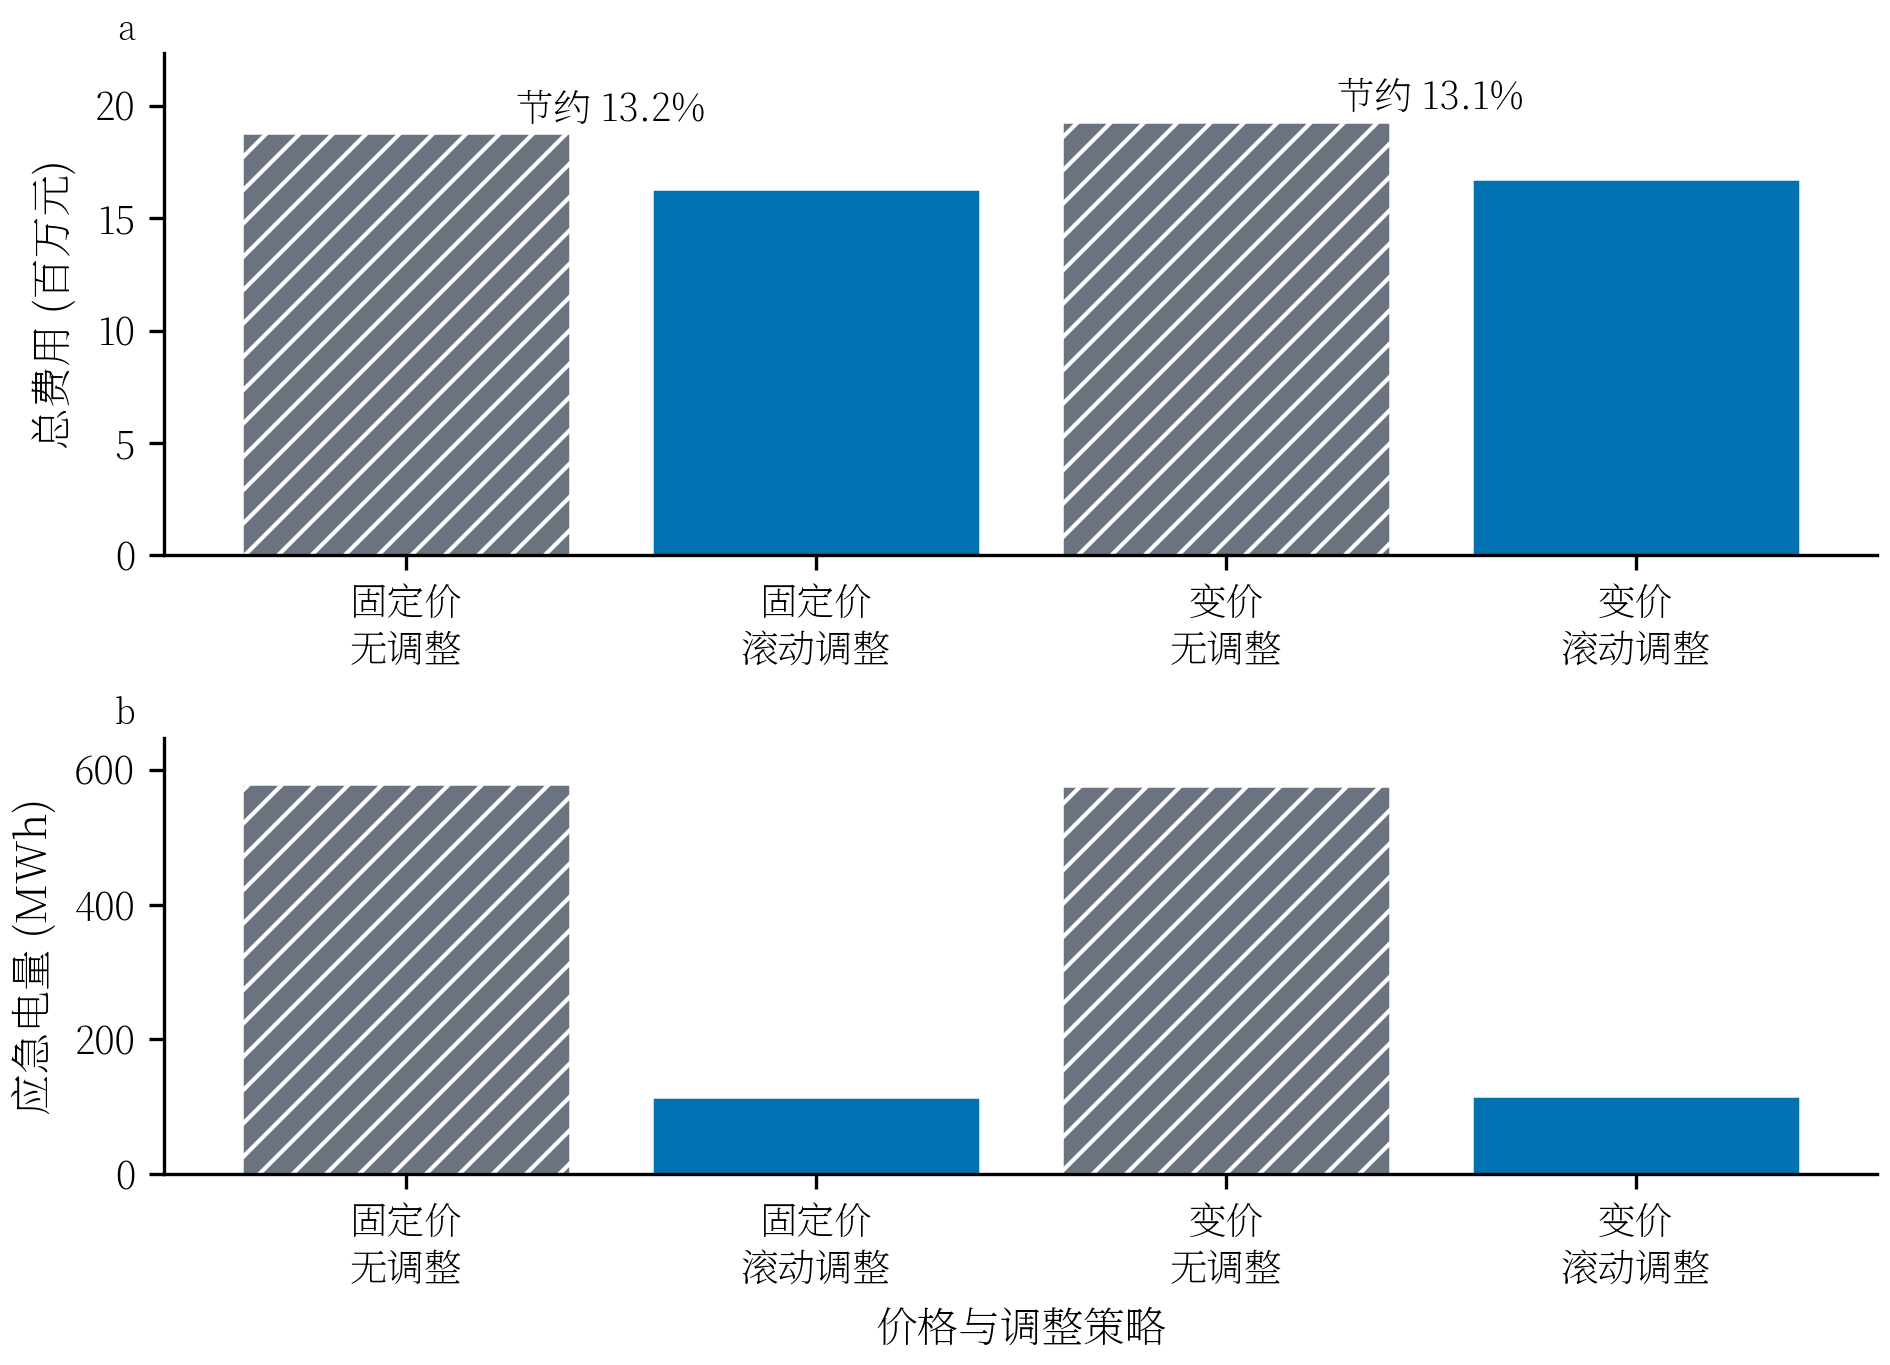
\includegraphics[width=0.96\textwidth]{figs/result_q4_strategy_comparison.png}
  \caption{固定价与变动电价下四个主策略的334日费用和应急购电量。}
  \label{fig:q4-result}
\end{figure}

代表日同样并非全部改善：12月21日无调账方案费用为 $74025.4512$ 元，有调账方案反而为 $77842.3118$ 元。其应急电量由 $382.2268$ 变为 $978.6827\,\mathrm{kWh}$。这说明滚动预测在总体上更有效，却可能在个别日期因预报误差、储能边界和价格预测偏差叠加而失利。两方案的完整代表日指定表见附录\ref{app:tables}和配套工作簿。

\subsection{变价条件下的更新频率建议}

在相同0时信息下，变价2小时合成更新方案费用为 $16033486.6253$ 元，6小时方案为 $16735118.3246$ 元，前者节约 $701631.6992$ 元，即4.1926\%。两方案相差2672次更新，故净收益为
\begin{equation}
 B^{\mathrm{var}}_{2h}=701631.6992-2672k,
 \label{eq:breakeven-variable}
\end{equation}
盈亏平衡阈值为 $262.5867$ 元/次。若采用替代结算式\eqref{eq:settlement-alt}对同一策略重计费，节约额缩小为 $139845.6748$ 元，不能把主结算阈值直接移用于该口径。

因此，问题四的建议为：在题设主结算解释成立、能够可靠取得最新官方预报和已观测前缀，且单次增量更新成本低于约262.59元时，可采用2小时合成更新；否则6小时官方发布节奏具有更稳健的实施性。2小时结果仅表示本题数据上的因果短临更新价值，不代表系统获得了额外官方预报产品。
